\documentclass{article}
\usepackage{amsmath}
\usepackage{amssymb}
\usepackage[svgnames]{xcolor}
\usepackage{graphicx}
\usepackage{enumitem}
\usepackage{multicol}
\usepackage{bbm}

\title{Computer Graphics: Assignment 03} % Title

\author{Lina Gundelwein, Letitia Parcalabescu, Anushalakshmi Manila} % Author name

\date{\today} % Date for the report

\begin{document}

\maketitle 

\section*{1. BRDF} 

\begin{itemize}
\item The three parameters which can be input into a BRDF are,
\begin{itemize}
\item Incoming light direction
\item Outgoing view direction 
\item Surface position 
\end{itemize}

\item The value of a BRDF for a certain parameter set tells us how much light is reflected when light makes contact with a certain material. \\

\item Either of the below two approaches could be used to obtain BRDFs.
\begin{itemize}
	\item  Use a device called gonioreflectometer to measure BRDF directly
	\item  Theoretical models such as Basis illumination approach for instance.
\end{itemize}

\end{itemize}

\section*{2. Aliasing} 
\begin{itemize}
\item Equation for the sampling frequency $w_s$ that is needed to reconstruct X(jw) with respect to $w_n$ is, $ w_s = 2*w_n$
\item Sampled signal with aliasing and without aliasing:\\
\includegraphics[width=0.9\textwidth]{aliasing.jpg}\\
\item Box filter can be used to reconstruct the original signal as sketched in the above diagram.
\[   
f(x) = 
\begin{cases}
\text{1,} &\quad\text{if x} \ge-1 \text{ and x}\le1\\
\text{0,} &\quad\text{otherwise.} \ 
\end{cases}
\]

\end{itemize}


\section*{3. Transformations} 


Matrix A scales by $0.5$ in y direction and mirrors about the y axis and matrix B mirrors about the zero crossing as depicted in the below diagram. \\
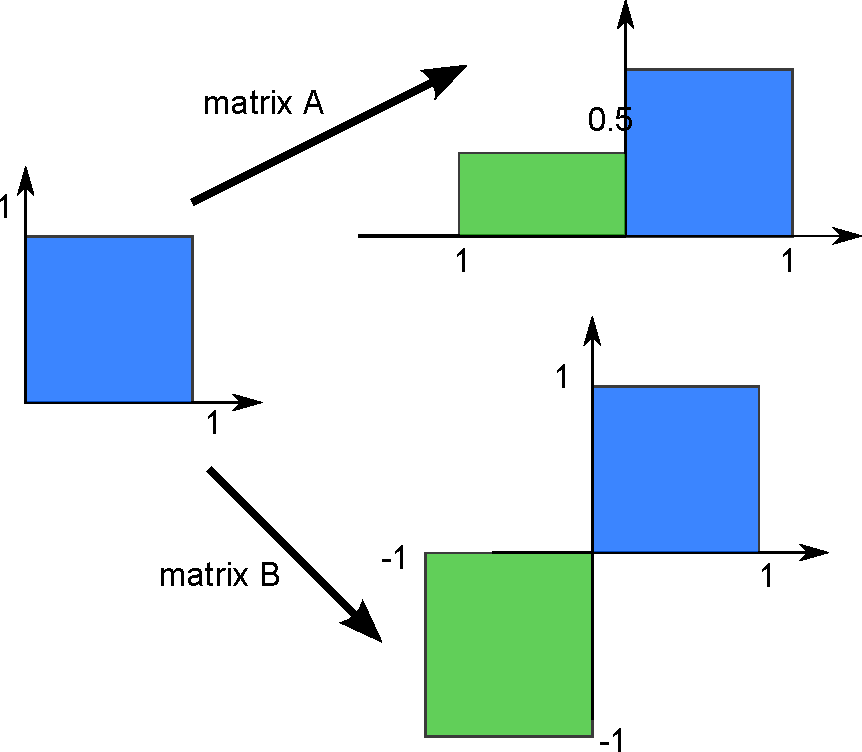
\includegraphics[width=0.5\linewidth]{drawing.png} \\

\begin{itemize}
\item Rotating an object without translating it equals a translation around the coordinate center.
\item Rotating after translating the center of the rectangle to zero results in a rotation around the rectangle center. (And a translation of (-3,2) if it is not translated back afterwards).
\item Rotating after tranlation of $V_1$ to the coordinate center will result in the rectangle rotated around $V_1$ and shifted by (-2,2).
\item Yes it is possible if you work with homogeneous coordinates. Transform vertices to homogeneous coordinates ($(2,2) \rightarrow (2,2,1)$ etc.) and multiply with matrix
\begin{equation*}
P = 
\begin{pmatrix}
1 & 0 &2\\
0 & 1 & 2\\
0 & 0 & 1
\end{pmatrix}
\begin{pmatrix}
\frac{\sqrt{2}}{2} & - \frac{\sqrt{2}}{2} & 0\\
\frac{\sqrt{2}}{2} &  \frac{\sqrt{2}}{2} & 0\\
0 & 0 & 1
\end{pmatrix}
\begin{pmatrix}
1 & 0 &-2\\
0 & 1 &-2\\
0 & 0 & 1
\end{pmatrix}=
\begin{pmatrix}
\frac{\sqrt{2}}{2} & - \frac{\sqrt{2}}{2} & 2\\
\frac{\sqrt{2}}{2} &  \frac{\sqrt{2}}{2} & 2-2\sqrt{2}\\
0 & 0 & 1
\end{pmatrix}\,.
\end{equation*}
\end{itemize}
\end{document}